
The directivity of a loudspeaker is a daily issue for sound events, because the loudspeaker produce sound outside the voluntary audience area. The sound from a speaker can therefore be defined as two main subject, sound for voluntary audience and sound for non voluntary audience, which is perceived the sound as noise. The following \autoref{fig:Problem} visualise the problem.


\begin{figure}[htbp]
	\centering
	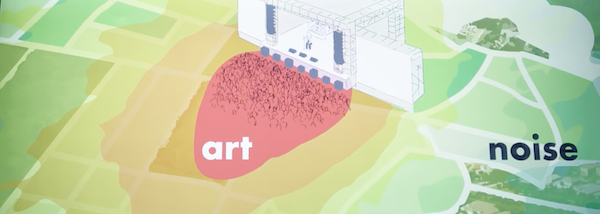
\includegraphics[width=1\textwidth]{change_later.png}
	\caption{Normalized \gls{spl} in colour, red is high \gls{spl} where blue is low \gls{spl}}
		\label{fig:Problem}
\end{figure}

\autoref{fig:Problem} shows the total sound pressure level \gls{spl} in \gls{db} from \SI{20}{\hertz} to \SI{20}{\kilo\hertz} for the voluntary audience and the non voluntary audience doing a concert. The voluntary audience condensing area is defined as participants area and is limited by the red area in figure \autoref{fig:Problem}. The non voluntary audience will be exposed by sound in a limited frequency area, when they are located outside but still in the neighbourhood of the red area. This area is defined as the neighbourhood area. The noise is cause by omnidirectionality of the line source module and have a limited frequency range. 

The directivity control of mid- and high frequency have a known solution which have been applied for many years. The solution is a horn design which is designed for a defined radiation pattern. Due to the long wave length in low/mid- and low frequency range, the horn principle will become a heavy solution for long wave length. Therefore other space saving solution have been analysed and implemented for about one decade. The commonly space saving solution is one subwoofer pointing forward and one subwoofer pointing backward with signalprocessing applied. This solution is both made by one box and two boxes.


This project aims to apply a new principle from D\&B audiotechnik SL-series, where the low/mid frequency directivity is controlled by signal processing tree speaker unit. One unit arranged in the front and two arranged on the side of the line source module, one on each side.



\section{preliminary problem statement}
The following questions are made with the intention of gathering the necessary knowledge, to be able to answer a later stated problem statement. The preliminary questions, which will be answered in the analysis, are:

\begin{itemize}
\item In which frequency area do the line source speaker behave omnidirectional?
\item Which known technique is used to do the speaker cardioid?
\item Can a simulation be made which support D\&B audiotechnik claim?
\end{itemize}



